\documentclass[tikz,border=3mm]{standalone}

\usepackage{amsmath}

\usetikzlibrary{matrix,positioning,fit,backgrounds,intersections, calc}



\begin{document}
\def\layersep{3.0cm}
%\begin{minipage}{0.6\columnwidth}
    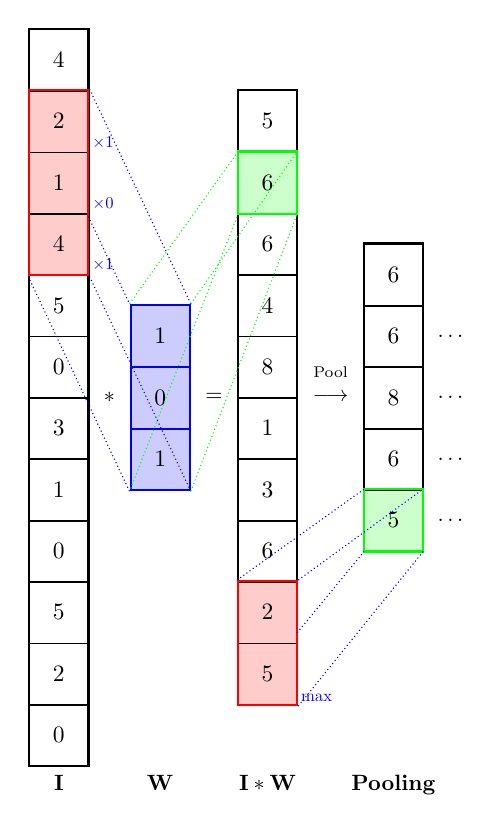
\begin{tikzpicture}[draw=black!50, mmat/.style={matrix of math nodes,column sep=-\pgflinewidth/2,
       row sep=-\pgflinewidth/2,cells={nodes={draw,inner sep=10pt,ultra thin, scale=0.85}},draw=#1,thick,inner sep=0pt},
       mmat/.default=black,
       node distance=0.3em,
       transform shape,scale=0.8]
    
    
    \tikzstyle{every pin edge}=[<-,shorten <=1pt]
    \tikzstyle{neuron}=[circle,fill=black!25,minimum size=10pt,inner sep=0pt]
    \tikzstyle{input neuron}=[neuron, fill=red!50];
    \tikzstyle{output neuron}=[neuron, fill=green!50];
    \tikzstyle{hidden neuron}=[neuron, fill=blue!50];
    \tikzstyle{annot} = [text width=4em, text centered]
    
    
    
     \matrix[mmat](mat1){
            {\scriptsize 4} \\ 
            {\scriptsize 2} \\ 
            {\scriptsize 1} \\ 
            {\scriptsize 4} \\ 
            {\scriptsize 5} \\ 
            {\scriptsize 0} \\ 
            {\scriptsize 3} \\
            {\scriptsize 1} \\
            {\scriptsize 0} \\
            {\scriptsize 5} \\
            {\scriptsize 2} \\
            {\scriptsize 0} \\
            };
     \def\myarray{{1},{0},{1}}       
    \foreach \Y in {0,1,2}
        {\foreach \X in {0}
            {\pgfmathsetmacro{\myentry}{{\myarray}[\Y][\X]}
            \path (mat1-\the\numexpr\Y+2\relax-1.south east)
            node[anchor=south west,blue,scale=0.75,inner sep=2.2pt]{$\times\myentry$};
    }}         
    \node[fit=(mat1-2-1)(mat1-4-1),inner sep=0pt,draw,red,thick,name path=fit](f1){};      
    \node[right=of mat1] (mul) {$*$};      
    \matrix[mmat=blue,fill=blue!20,right=of mul,name path=mat2](mat2){    
        1 \\ 
        0 \\ 
        1 \\ };
    \node[right=of mat2] (eq) {$=$};       
    \matrix[mmat,right=of eq](mat3){
        5 \\
        |[alias=4]|6 \\ 
        6 \\ 
        4 \\ 
        8 \\ 
        1 \\
        3 \\
        6 \\
        2 \\
        5 \\
    };
    \node[fit=(mat3-2-1)(mat3-2-1),inner sep=0pt,draw,green,thick,name path=not_to_consider](ntc){};
    \node[fit=(mat3-9-1)(mat3-10-1),inner sep=0pt,draw,red,thick,name path=fit2](f2){};
    \node[right=of mat3, label={\scriptsize Pool}] (pool) {$\longrightarrow$};
    \matrix[mmat,right=of pool,name path=mmat3](mat4){    
        6 \\ 
        6 \\ 
        8 \\
        6 \\
        |[alias=2]|5 \\
    };
    \node[fit=(mat4-5-1)(mat4-5-1),inner sep=0pt,draw,green,thick,name path=fit3](f3){};
%   \node[right=of mat4-1-1, label={\scriptsize DNN}] (DNN1) {$\longrightarrow$};
   \node[right=of mat4-2-1] (DNN2) {$\dots$};
   \node[right=of mat4-3-1] (DNN3) {$\dots$};
   \node[right=of mat4-4-1] (DNN4) {$\dots$};
   \node[right=of mat4-5-1] (DNN5) {$\dots$};
    
    
    
    \foreach \Anchor in {south west,north west,south east,north east}
     {\path[name path=test] (f1.\Anchor) -- (mat2.\Anchor);
     \draw[blue,densely dotted,name intersections={of=test and fit,total=\t}]
     \ifnum\t>0 (intersection-\t) -- (mat2.\Anchor) \else
      (f1.\Anchor) -- (mat2.\Anchor)\fi;
      
     \path[name path=test2]  (4.\Anchor) -- (mat2.\Anchor);  
     \draw[green,densely dotted,name intersections={of=test2 and mat2,total=\tt}] 
     \ifnum\tt>0 (intersection-1) -- (4.\Anchor) \else
        (mat2.\Anchor) --  (4.\Anchor)\fi;
    
     \path[name path=test3] (f2.\Anchor) -- (mat4.\Anchor);
     \draw[blue,densely dotted,name intersections={of=test3 and fit2,total=\t}]
     \ifnum\t>0 (intersection-\t) -- (2.\Anchor) \else
      (f2.\Anchor) -- (2.\Anchor)\fi;
        }
        
     \path (mat3-10-1.south east) node[anchor=south west,blue,scale=0.75,inner sep=2.2pt]{max};
     \path (mat1.south) node[below] {$\mathbf{I}$}
      (mat2|-mat1.south) node[below] {$\mathbf{W}$}
      (mat3|-mat1.south) node[below] {$\mathbf{I}*\mathbf{W}$}
      (mat4|-mat1.south) node[below] {\textbf{Pooling}};

   \begin{scope}[on background layer]
       \fill[red!20] (f1.north west) rectangle (f1.south east);
   \end{scope}
    \begin{scope}[on background layer]
        \fill[red!20] (f2.north west) rectangle (f2.south east);
    \end{scope}
    \begin{scope}[on background layer]
        \fill[green!20] (ntc.north west) rectangle (ntc.south east);
    \end{scope}
    \begin{scope}[on background layer]
        \fill[green!20] (2.north west) rectangle (2.south east);
    \end{scope}

\end{tikzpicture}%%%%%%%%%%%%%%%%%%%%%%%%%%%%%%%%%%%%%%%%%%%%%%%%%
\end{document}
